\chapter{\label{ChapterAdaptiveMLEnOptAlgorithm}Adaptive‑ML‑EnOpt algorithm}

In this chapter, we describe the Adaptive-ML-EnOpt algorithm \cite{Keil2022-dj}, which is a modified version of the EnOpt algorithm. This algorithm is supposed to reduce the number of FOM evaluations by using a machine learning-based surrogate functional, which improves the computation speed with respect to the EnOpt algorithm. Therefore, we introduce deep neural networks (DNNs) next. After that, the Adaptive-ML-EnOpt-algorithm is presented.

\section{\label{sectionDeepNeuralNetworks}Deep neural networks}

This description of deep neural networks is based on the definitions in \cite{Keil2022-dj}.

DNNs are used here to approximate a function $f:\mathbb{R}^{N_{\mathrm{in}}}\to\mathbb{R}^{N_{\mathrm{out}}}$ with $N_{\mathrm{in}},N_{\mathrm{out}}\in\mathbb{N}$. We call $L\in\mathbb{N}$ the number of layers and $N_{\mathrm{in}}=N_0,N_1,\dotsc,N_{L-1}, N_L=N_{\mathrm{out}}$ the numbers of neurons in each layer. We refer to the layers $1$ to $L-1$ as the hidden layers. $W_i\in\mathbb{R}^{N_i\times N_{i-1}}$ denotes the weights in layer $i\in\{1,\dotsc,L\}$ and $b_i\in\mathbb{R}^{N_i}$ the biases of the layer $i\in\{1,\dotsc,L\}$. These are composed as $\mathbf{W}=\left((W_1,b_1),\dotsc,(W_L,b_L)\right)$, which is a tuple of pairs of corresponding weights and biases.

$\rho:\mathbb{R}\to\mathbb{R}$ is the so-called activation function. A popular example is the rectified linear unit funtion $\rho(x)=\operatorname{max}(x,0)$, however we will use the hyperbolic tangent funtion
\begin{displaymath}
\rho(x)=\tanh(x)=\frac{\exp(2x)-1}{\exp(2x)+1}.
\end{displaymath}
$\rho_n^*:\mathbb{R}^n\to\mathbb{R}^n$ is now defined as the component-wise application of $\rho$ onto a vector of dimension $n$, so $\rho_n^*(x)=\left[\rho(x_1),\dotsc,\rho(x_n)\right]^T$ for $x\in\mathbb{R}^n$.

To calculate the output $\Phi_\mathbf{W}(x)\in\mathbb{R}^{N_{\mathrm{out}}}$ of a DNN for an input $x\in\mathbb{R}^{N_{\mathrm{in}}}$, we apply the weights, biases, and activation function multiple times onto the input. It is computed iteratively with the functions $r_0:\mathbb{R}^{N_0}\to\mathbb{R}^{N_0}$ and $r_i:\mathbb{R}^{N_{i-1}}\to\mathbb{R}^{N_i}$ for $i=1,\dotsc,L$ by
\begin{eqnarray*}
r_0(x)&:=&x,\\
r_i(x)&:=&\rho_{N_i}^*(W_ir_{i-1}(x)+b_i)\text{ for }i=1,\dotsc,L-1,\\
r_L(x)&:=&W_Lr_{L-1}(x)+b_L,\\
\Phi_\mathbf{W}(x)&:=&r_L(x).
\end{eqnarray*}

Now we try to optimize the parameters in $\mathbf{W}$ such that $\Phi_\mathbf{W}\approx f$. To achieve this, we sample a set that consists of inputs $x_i\in X\subset\mathbb{R}^{N_{\mathrm{in}}}$ and corresponding outputs $f(x_i)\in\mathbb{R}^{N_{\mathrm{out}}}$ and assemble them in the so-called training set
\begin{equation}
T_\mathrm{train}=\{(x_1,f(x_1)),\dotsc,(x_{N_\mathrm{train}},f(x_{N_\mathrm{train}}))\}\subset X\times\mathbb{R}^{N_\mathrm{out}}.
\end{equation}
To evaluate the performance of our chosen $\mathbf{W}$, we use the mean squared error loss $\mathscr{L}(\Phi_\mathbf{W},T_\mathrm{train})$ to measure the distance between $\Phi_\mathbf{W}$ and $f$ on a training set. The mean squared error loss is defined as
\begin{displaymath}
\mathscr{L}(\Phi_\mathbf{W},T_\mathrm{train}):=\frac{1}{|T_\mathrm{train}|}\sum_{(x,y)\in T_\mathrm{train}}\| \Phi_\mathbf{W}(x)-y\|_2^2.
\end{displaymath}
Since we want $\Phi_\mathbf{W}$ to be close to $f$, we minimize the loss function with respect to $\mathbf{W}$. For that, we use some gradient-based optimization method. By the structure of the neural network, we can use the chain rule multiple times to divide the gradient of $\mathscr{L}$ into much simpler gradient computations.\\

We want that $\Phi_\mathbf{W}$ is close to $f$ on $X$ but we train it only on a sample set of $X$, so we achieve that $\Phi_\mathbf{W}$ is only on $T_\mathrm{train}$ close to $f$. During the training, the loss function will eventually decrease on the training set, but at some point the loss on different samples, that are not in the training set, will get worse \cite{Prechelt2012}. This is called 'overfitting'.

To prevent overfitting, we use early stopping. For early stopping, we evaluate the loss function on a validation set $T_\mathrm{val}\subset X\times\mathbb{R}^{N_\mathrm{out}}$, where usually $T_\mathrm{val}\cap T_\mathrm{train}=\emptyset$. Our algorithm for early stopping is described in the following.\\

For that, let $\mathbf{W}^{(k)}$ be the weights in epoch $k$. To evaluate the quality of the neural network that results from $\mathbf{W}^{(k)}$, the MSE loss on the validation set $\mathscr{L}(\Phi_{\mathbf{W}^{(k)}},T_\mathrm{val})$ is computed at the end of each training epoch. Now let $k_0$ be the iteration where $\mathbf{W}^{(k_0)}$ is smaller than the losses in all previous iterations. If that is the case, we save $\mathbf{W}^{(k_0)}$ and its corresponding loss $\mathscr{L}(\Phi_{\mathbf{W}^{(k_0)}},T_\mathrm{val})$. In the next $k^*$ iterations, where $k^*$ is a prescribed number, we check if $\mathscr{L}(\Phi_{\mathbf{W}^{(k_0+i)}},T_\mathrm{val})<\mathscr{L}(\Phi_{\mathbf{W}^{(k_0)}},T_\mathrm{val})$ for $i=1,\dotsc,k^*$. If that is the case for some $i$, we update $\mathbf{W}^{(k_0)}$ and $\mathscr{L}(\Phi_{\mathbf{W}^{(k_0)}},T_\mathrm{val})$ by setting them to $\mathbf{W}^{(k_0+i)}$ and $\mathscr{L}(\Phi_{\mathbf{W}^{(k_0+i)}},T_\mathrm{val})$. Then the last step is repeated. If there is no such $i$ between $1$ and $k^*$, the training is aborted and the last saved weights returned.

So we abort the training if the minimum loss is not decreasing over a prescribed number of consecutive epochs. Our reasoning behind this is that the loss on the validation set is not srictly decreasing and can even increase over some epochs, but that is fine for us as long as we can decrease the loss over time.

Figure \ref{earlyStoppingPlot} shows an example where we used early stopping with $k^*=15$. Here, the validation loss of the last training epochs is presented. We see that a minimum is reached after $44$ iterations. Since the next $15$ training epochs yield no decrease of the MSE loss, the training is aborted after iteration $59$.\\

\begin{figure}
\centering
%\textbf{Your title}\par\medskip
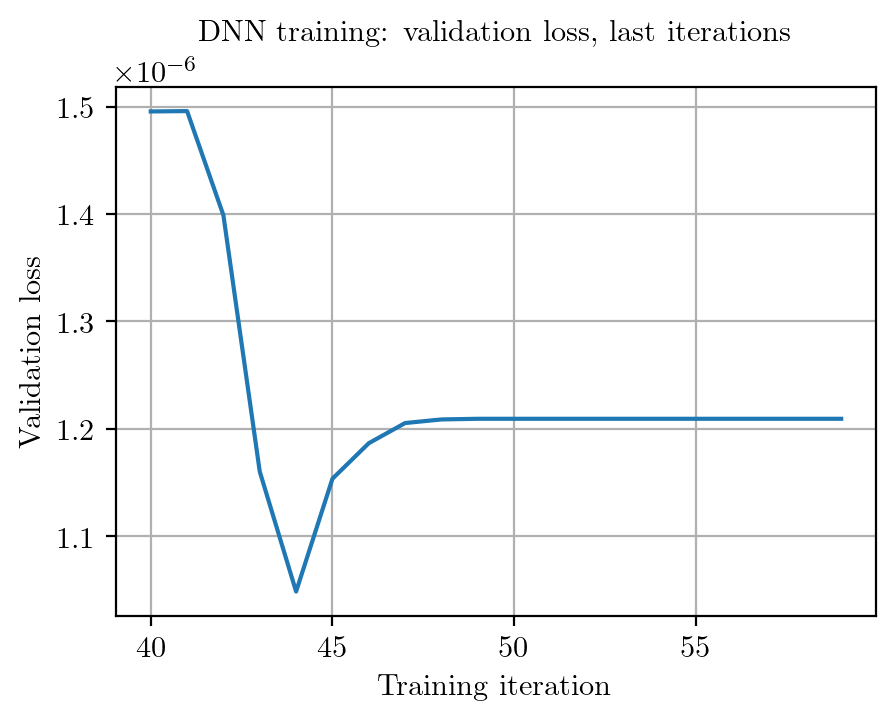
\includegraphics{Plots/earlyStopping.png}
\caption{\label{earlyStoppingPlot}Validation loss during the last iterations of a neural network training procedure where early stopping was applied}
\end{figure}

We present now the construction of a DNN that approximates a function $f:\mathbb{R}^n\to\mathbb{R}$ with $n\in\mathbb{N}$. The training of one neural network is shown in algorithm \ref{trainDNN}. It takes the initialization of the deep neural network ($\mathrm{DNN}$), the inputs and outputs of the training set ($x_\mathrm{train}, y_\mathrm{train}$), the inputs and outputs of the validation set ($x_\mathrm{val}, y_\mathrm{val}$), the loss function ($\textproc{loss\_fn}$), the optimizer ($\mathrm{optimizer}$), the number of training epochs ($\mathrm{epochs}$) and the number ($\mathrm{earlyStop}$) that describes after how many iterations without improvement of the validation loss the training gets aborted, so that is the $k^*$ from above.

In our algorithm, the loss function is chosen as the mean squared error loss and we use the L-BFGS algorithm \cite{Liu1989-ua}, which is a limited memory quasi-Newton method that uses approximations of the objective functions Hessian matrix, with strong Wolfe line-search \cite{doi:10.1137/1011036, doi:10.1137/1013035} as our optimizer. The number of training epochs is only the maximum number of iterations since we apply early stopping to our training algorithm. Usually, the training terminates earlier because the loss over the validation set is not decreasing further.

The function $\textproc{testDNN}$ in algorithm \ref{trainDNN} returns the loss of the function $\textproc{loss\_fn}$ between the output of the DNN with the current parameters and the output of the objective function over the validation set which is denoted by $y_\mathrm{val}$. So if $\textproc{loss\_fn}=\mathscr{L}$, we have $\textproc{testDNN}(\textproc{DNN}, x_\mathrm{val}, y_\mathrm{val}, \textproc{loss\_fn}) = \mathscr{L}(\mathrm{DNN}, T_\mathrm{val})$ with
\begin{displaymath}
T_\mathrm{val}=\{((x_\mathrm{val})_1,(y_\mathrm{val})_1),\dotsc,((x_\mathrm{val})_{N_\mathrm{val}},(y_\mathrm{val})_{N_\mathrm{val}})\}.
\end{displaymath}

In addition, some funtions are imported from the Python package PyTorch. These functions are identified by the beginning `$\mathrm{torch.}$'.

\begin{algorithm}[H]%\footnotesize
\caption{\label{trainDNN}DNN training}
\begin{algorithmic}[1]
\Function{trainDNN}{$\textproc{DNN}, x_\mathrm{train}, y_\mathrm{train}, x_\mathrm{val}, y_\mathrm{val}, \textproc{loss\_fn}, \mathrm{optimizer}, \mathrm{epochs}, \mathrm{earlyStop}$}
\State $\mathrm{wait} \gets 0$
\State $\mathrm{minimalValidationLoss} \gets \Call{testDNN}{\mathrm{DNN}, x_\mathrm{val}, y_\mathrm{val}, \textproc{loss\_fn}}$
%\State \text{save the current parameters of the DNN}%$\mathrm{torch.save}(\mathrm{DNN.state\_dict}(), \mathrm{'checkpoint.pth'})$
\State $\mathrm{torch.}\Call{save}{\textproc{DNN.}\protect\Call{state\_dict}{\:}, \mathrm{'checkpoint.pth'}}$
\For{$\mathrm{epoch}=1,\dotsc,\mathrm{epochs}$}
%\State \text{do one training step with the }$\mathrm{optimizer}$
\State\label{startTrainStep} $\textproc{DNN.}\Call{train}{\:}$
\Function{closure}{\:}
    \State $\mathrm{y\_pred} \gets \Call{DNN}{\mathrm{x\_train}}\Call{.reshape}{\protect\Call{len}{\mathrm{y\_train}}}$
    \State $\mathrm{loss} \gets \Call{loss\_fn}{\mathrm{y\_pred}, \mathrm{y\_train}}$
    \State $\mathrm{optimizer.}\Call{zero\_grad}{\:}$
    \State $\mathrm{loss.}\Call{backward}{\:}$
    \State \Return $\mathrm{loss}$
\EndFunction
\State\label{endTrainStep} $\mathrm{optimizer.}\Call{step}{\textproc{closure}}$
\State $\mathrm{validationLoss} \gets \Call{testDNN}{\textproc{DNN}, x_\mathrm{val}, y_\mathrm{val}, \textproc{loss\_fn}}$
\If{$\mathrm{validationLoss} < \mathrm{minimalValidationLoss}$}
\State $\mathrm{wait} \gets 0$
\State $\mathrm{minimalValidationLoss} \gets \mathrm{validationLoss}$
%\State \text{save the current parameters of the DNN}%$\mathrm{torch.save}(\mathrm{DNN.state\_dict}(), \mathrm{'checkpoint.pth'})$
\State $\mathrm{torch.}\Call{save}{\textproc{DNN.}\protect\Call{state\_dict}{\:}, \mathrm{'checkpoint.pth'}}$
\Else
\State $\mathrm{wait} \gets \mathrm{wait}+1$
\EndIf
\If{$\mathrm{wait} \geq \mathrm{earlyStop}$}
%\State \text{overwrite the parameters of the DNN with the saved parameters}%$\mathrm{DNN.load\_state\_dict}(\mathrm{torch.load}(\mathrm{'checkpoint.pth'}))$
\State $\textproc{DNN.}\Call{load\_state\_dict}{\mathrm{torch.}\protect\Call{load}{\mathrm{'checkpoint.pth'}}}$
\State \Return
\EndIf
\EndFor
\EndFunction
\end{algorithmic}
\end{algorithm}

We start the algorithm $\textproc{trainDNN}$ by initializing the variable $\mathrm{wait}$, which indicates the number of training epochs without a decrease of the loss on the evaluation set, as zero and the variable $\mathrm{minimalValidationLoss}$, which shows the loss that was achieved '$\mathrm{wait}$' epochs ago, as the loss on the validation set for the DNN before the training begins. Then the weights and biases of the DNN are saved in the file `$\mathrm{checkpoint.pth}$'. After that, the following operations are executed in every training epoch.

The procedures that are performed between line \ref{startTrainStep} and line \ref{endTrainStep} can be described as doing one optimization step with the $\mathrm{optimizer}$ to decrease the loss on the training set by adjusting the weights and biases of the DNN. Then we check if the loss on the evaluation set is currently smaller than the minimal validation loss over all previous epochs.

If that is the case, the variable $\mathrm{wait}$ is set to zero, indicating that the current parameters of the DNN have the best performance over the validation set, and the variable $\mathrm{minimalValidationLoss}$ is updated to the current validation loss. Since the parameters of the DNN will be changed in the next epochs, the current weights and biases are saved again in the file `$\mathrm{checkpoint.pth}$'. If the validation loss is not less than the minimal validation loss, the variable $\mathrm{wait}$ is increased by one.

To implement early stopping as described above, we check at the end of each training epoch whether the minimum loss has not decreased over so many consecutive epochs that we terminate the algorithm prematurely. If $\mathrm{wait} \geq \mathrm{earlyStop}$, the current parameters of the neural network are overwritten with the parameters that were saved when the minimum loss was reached and the algorithm is aborted.\\

Since we search for local minima of the loss function, the initial value $\mathbf{W}^{(0)}$ of our iteration effects the local optimum that we get and therefore the performance. We use Kaiming initialization \cite{7410480} to set our initial value $\mathbf{W}^{(0)}$. With Kaiming initialization, the starting values are initialized randomly since the elements of the weights $W_i$ are sampled from a zero-mean Gaussian distribution whose standard deviation is $\sqrt{2/N_{i-1}}$ for $i\in\{1,\dotsc,L\}$.
%The biases $b_i$ are set to zero for $i\in\{1,\dotsc,L\}$. 
The idea behind this type of random sampling is that the specified standard deviation prevents the exponential increase/ reduction of the input as shown in \cite{7410480}.

For the training of the DNN, we perform multiple restarts of the training algorithm with different initializations of $\mathbf{W}^{(0)}$ which minimizes the dependence of our neural network from the initial values. After we have trained enough DNNs, we select the neural network $\Phi_{\mathbf{W}^*}$ that has the smallest evaluation loss $\mathscr{L}(\Phi_{\mathbf{W}^*},T_\mathrm{val})$ over all restarts.

Figure \ref{DNNRestartsPlot} shows that training multiple neural networks can help to reduce the validation loss. If we did not restart the training, our DNN would have a validation loss of slightly above $3\cdot10^{-6}$. After two restarts, we obtain a neural network with a validation loss that is less than half of the DNN with no restarts. Of course, there are iterations where repeating the training does not lead to a reduction of the validation loss, but in general, the more neural networks we train, the lower the resulting loss tends to be. However, training more DNNs also increases the runtime.\\

\begin{figure}
\centering
%\textbf{Your title}\par\medskip
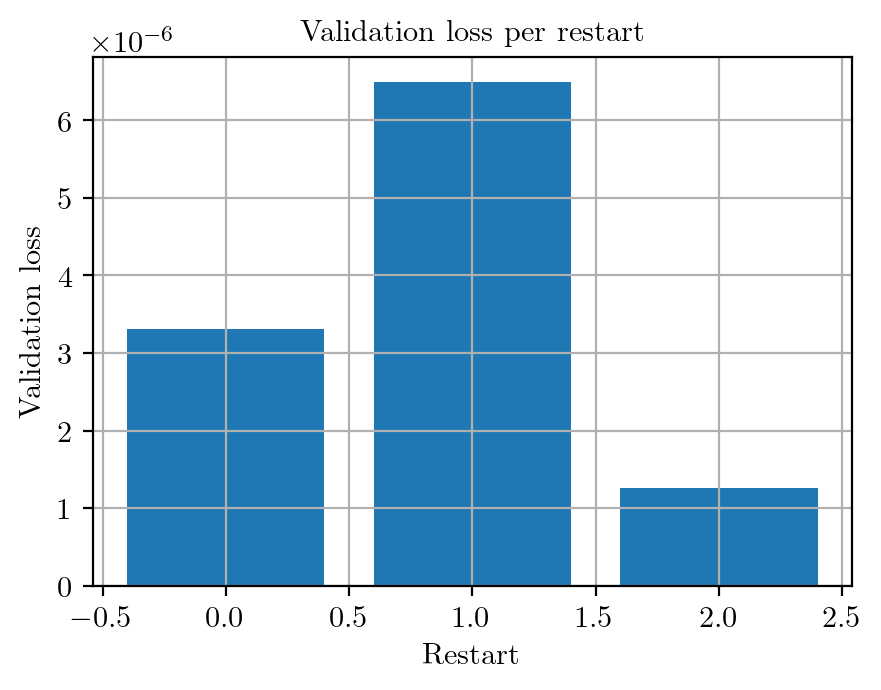
\includegraphics{Plots/DNNRestarts.png}
\caption{\label{DNNRestartsPlot}Example of the different validation losses resulting from the training of three neural networks}
\end{figure}

Before the whole algorithm for the construction of the DNN is presented, we look at the data that we use for the training. If we sample the inputs in a small area, it is likely that the corresponding outputs are also close to each other. Since we convert the values for the training of the neural network from 64-bit floating point numbers to 32-bit floating point numbers, it can even happen that the converted inputs or outputs are constant. In that case, the digits of these values that differ from each other get cut off at the conversion.

We want the values of the inputs and outputs to be distributed in such a way that significant differences are correctly represented. For that, the inputs $x\in\mathbb{R}^n$ and outputs $y\in\mathbb{R}$ are scaled to $\tilde{x}\in[0,1]^n$ and $\tilde{y}\in[0,1]$.

Let
\begin{equation}
T=\{(x_1,y_1),\dotsc,(x_N,y_N)\}
\end{equation}
be a sample set of size $N$ and
\begin{align*}
T_x&=\{x_1,\dotsc,x_N\},&T_y&=\{y_1,\dotsc,y_N\}
\end{align*}
the sets that contain the inputs and outputs of that sample.

We define $x^\mathrm{low}, x^\mathrm{upp}\in\mathbb{R}^n$ and $y^\mathrm{low}, y^\mathrm{upp}\in\mathbb{R}$ as
\begin{eqnarray}
\label{minIn}
x^\mathrm{low}_i&:=&\operatorname*{min}\{x_i\mid x\in T_x\}\text{ for }i=1,\dotsc,n,\\
\label{maxIn}
x^\mathrm{upp}_i&:=&\operatorname*{max}\{x_i\mid x\in T_x\}\text{ for }i=1,\dotsc,n,\\
\label{minOut}
y^\mathrm{low}&:=&\operatorname*{min}T_y,\\
\label{maxOut}
y^\mathrm{upp}&:=&\operatorname*{max}T_y.
\end{eqnarray}

Now, $\tilde{x}$ and $\tilde{y}$ are calculated as
\begin{align}
\label{scalingToZeroOne}
\tilde{x}_i&=\frac{x_i-x^\mathrm{low}_i}{x^\mathrm{upp}_i-x^\mathrm{low}_i}\text{ for }i=1,\dotsc,n,&\tilde{y}&=\frac{y-y^\mathrm{low}}{y^\mathrm{upp}-y^\mathrm{low}}.
\end{align}

After we have trained the neural network, the DNN outputs need to be rescaled so that we get a proper approximation of the function $f$. The output $\Phi(\tilde{x})$ of the DNN $\Phi$ is rescaled with the calculation $\Phi(\tilde{x})\cdot(y^\mathrm{upp}-y^\mathrm{low})+y^\mathrm{low}$.
%\begin{eqnarray*}
%\tilde{x}_i&=\frac{x_i-x^\mathrm{low}_i}{x^\mathrm{upp}_i-x^\mathrm{low}_i}&\text{ for }i=1,\dotsc,n,\\
%\tilde{y}&=\frac{y-y^\mathrm{low}}{y^\mathrm{upp}-y^\mathrm{low}},&
%\end{eqnarray*}

To summarize this, we present now the construction of a DNN as pseudo code in algorithm \ref{DNNConstruction}. Training parameters like the neural network structure ($\mathrm{DNNStructure}$), the activation function ($\textproc{activFunc}$), the number of restarts of different DNN initializations ($\mathrm{restarts}$), the number of training epochs ($\mathrm{epochs}$), the number of epochs without decrease of the evaluation loss after which early stopping is applied ($\mathrm{earlyStop}$), the fraction of the sample that is used for training ($\mathrm{trainFrac}$) and the learning rate ($\mathrm{learning\_rate}$) are stored in $V_\mathrm{DNN}$. We denote $x^\mathrm{low}$ as $\mathrm{minIn}$, $x^\mathrm{upp}$ as $\mathrm{maxIn}$, $y^\mathrm{low}$ as $\mathrm{minOut}$ and $y^\mathrm{upp}$ as $\mathrm{maxOut}$. $\mathrm{minIn}$ and $\mathrm{maxIn}$ are calculated before the construction of the DNN and are taken as an input. The function $\textproc{FullyConnectedNN}$ is imported from $\mathrm{pymor.models.neural\_network}$ which is included in the Python package pyMOR. It builds a neural network with Kaiming initialization where the number of neurons in each layer gets specified by the first and the activation function of the neural network by the second argument.

\begin{algorithm}[H]%\footnotesize
\caption{\label{DNNConstruction}DNN construction}
\begin{algorithmic}[1]
\Function{constructDNN}{$\mathrm{sample}, V_\mathrm{DNN}, \mathrm{minIn}, \mathrm{maxIn}$}
%\State \text{scale inputs and outputs like described and save them as }$\mathrm{normSample}$\text{ and }$\mathrm{normVal}$
\State $\mathrm{normSample} \gets \mathrm{np.}\Call{zeros}{\protect\Call{len}{\mathrm{sample}}, \protect\Call{len}{\mathrm{sample}[0][0]}}$
\State $\mathrm{normVal} \gets \mathrm{np.}\Call{zeros}{\protect\Call{len}{\mathrm{sample}}}$
\For{$i = 0,\dotsc,\Call{len}{\mathrm{sample}}-1$}
\State $\mathrm{normSample}[i, :] \gets \mathrm{sample}[i][0]$
\State $\mathrm{normVal}[i] \gets \mathrm{sample}[i][1]$
\EndFor
\State $\mathrm{minOut} \gets \mathrm{np.}\Call{min}{\mathrm{normVal}}$
\State $\mathrm{maxOut} \gets \mathrm{np.}\Call{max}{\mathrm{normVal}}$
%\State $\textproc{scaleInput} \gets \mathbf{lambda}\:\mathrm{mu}: (\mathrm{mu}-\mathrm{minIn})/(\mathrm{maxIn}-\mathrm{minIn})$
%\State $\textproc{scaleOutput} \gets \mathbf{lambda}\:\mathrm{mu}: (\mathrm{mu}-\mathrm{minOut})/(\mathrm{maxOut}-\mathrm{minOut})$
%\State $\textproc{rescaleOutput} \gets \mathbf{lambda}\:\mathrm{mu}: \mathrm{mu}\cdot(\mathrm{maxOut}-\mathrm{minOut})+\mathrm{minOut}$
%\State $\mathrm{normSample} \gets \Call{scaleInput}{\mathrm{normSample}}$
%\State $\mathrm{normVal} \gets \Call{scaleOutput}{\mathrm{normVal}}$
\State\label{inputScaling} $\mathrm{normSample} \gets (\mathrm{normSample}-\mathrm{minIn})/(\mathrm{maxIn}-\mathrm{minIn})$
\State\label{outputScaling} $\mathrm{normVal} \gets (\mathrm{normVal}-\mathrm{minOut})/(\mathrm{maxOut}-\mathrm{minOut})$
%\State \text{divide }$\mathrm{normSample}$\text{ and }$\mathrm{normVal}$\text{ into train/test splits }$x_\mathrm{train}, y_\mathrm{train}, x_\mathrm{val}, y_\mathrm{val}$
\State\label{tensorConversion1} $x \gets \mathrm{torch.}\Call{from\_numpy}{\mathrm{normSample}}\Call{.to}{\mathrm{torch.float32}}$
\State\label{tensorConversion2} $y \gets \mathrm{torch.}\Call{from\_numpy}{\mathrm{normVal}}\Call{.to}{\mathrm{torch.float32}}$
\State $\mathrm{trainSplit} \gets \Call{int}{\mathrm{trainFrac} * \protect\Call{len}{x}}$
\State $x_\mathrm{train}, y_\mathrm{train} \gets x[:\mathrm{trainSplit}], y[:\mathrm{trainSplit}]$
\State $x_\mathrm{val}, y_\mathrm{val} \gets x[\mathrm{trainSplit}:], y[\mathrm{trainSplit}:]$
\State $\textproc{DNN} \gets \Call{FullyConnectedNN}{\mathrm{DNNStructure}, \textproc{activation\_function}\gets\textproc{activFunc}}$
\State $\textproc{loss\_fn} \gets \mathrm{torch.nn.}\Call{MSELoss}{\:}$
\State $\mathrm{optimizer} \gets \mathrm{torch.optim.}\Call{LBFGS}{\protect\Call{DNN.parameters}{\:}, \mathrm{lr}\gets\mathrm{learning\_rate}, \mathrm{line\_search\_fn}\gets\mathrm{'strong\_wolfe'}}$
\State $\Call{trainDNN}{\textproc{DNN}, x_\mathrm{train}, y_\mathrm{train}, x_\mathrm{val}, y_\mathrm{val}, \textproc{loss\_fn}, \mathrm{optimizer}, \mathrm{epochs}, \mathrm{earlyStop}}$
\State\label{defEvalDNN} $\mathrm{evalDNN} \gets \Call{testDNN}{\textproc{DNN}, x_\mathrm{val}, y_\mathrm{val}, \textproc{loss\_fn}}$
\For{$i=1,\dotsc,\mathrm{restarts}$}
\State $\textproc{DNN}_i \gets \Call{FullyConnectedNN}{\mathrm{DNNStructure}, \textproc{activation\_function}\gets\textproc{activFunc}}$
\State $\mathrm{optimizer} \gets \mathrm{torch.optim.}\Call{LBFGS}{\protect\Call{DNN$_i$.parameters}{\:}, \mathrm{lr}\gets\mathrm{learning\_rate}, \mathrm{line\_search\_fn}\gets\mathrm{'strong\_wolfe'}}$
\State $\Call{trainDNN}{\mathrm{DNN}_i, x_\mathrm{train}, y_\mathrm{train}, x_\mathrm{val}, y_\mathrm{val}, \textproc{loss\_fn}, \mathrm{optimizer}, \mathrm{epochs}, \mathrm{earlyStop}}$
\State $\mathrm{evalDNN}_i \gets \Call{testDNN}{\textproc{DNN}_i, x_\mathrm{val}, y_\mathrm{val}, \textproc{loss\_fn}}$
\If{$\mathrm{evalDNN}_i<\mathrm{evalDNN}$}
\State $\mathrm{evalDNN} \gets \mathrm{evalDNN}_i$
\State $\mathrm{DNN} \gets \mathrm{DNN}_i$
\EndIf
\EndFor
%\State $F_\mathrm{ML} \gets \mathbf{lambda}\:\mathrm{mu}: \Call{rescaleOutput}{\protect\Call{DNN}{\protect\Call{scaleInput}{\mathrm{mu}}}}$
\Function{F$_\mathrm{ML}$}{$x_\mathrm{inp}$}
\State $\mathrm{scaledInput} \gets \mathrm{torch.}\Call{from\_numpy}{(x_\mathrm{inp}-\mathrm{minIn})/(\mathrm{maxIn}-\mathrm{minIn})}.\Call{to}{\mathrm{torch.float32}}$
%with torch.inference_mode():
\State $\mathrm{scaledOutput} \gets \Call{DNN}{\mathrm{scaledInput}}$
\State \Return $\mathrm{scaledOutput.}\Call{numpy}{\:}[0]\cdot(\mathrm{maxOut}-\mathrm{minOut})+\mathrm{minOut}$
\EndFunction
\State \Return $\textproc{F$_\mathrm{ML}$}$
\EndFunction
\end{algorithmic}
\end{algorithm}

The algorithm $\textproc{constructDNN}$ begins by setting the scaled samples for training and testing. For that, $\mathrm{normSample}$ is defined as a matrix where each row $i$ is equal to the input sample $\mathrm{sample}[i][0]$ and $\mathrm{normVal}$ is a vector where each element $i$ is set to the output sample $\mathrm{sample}[i][1]$. Then we scale and translate them in line \ref{inputScaling} and \ref{outputScaling} as it is shown in \eqref{scalingToZeroOne}.

After $\mathrm{normSample}$ and $\mathrm{normVal}$ are converted to a 32-bit floating point data type tensor from the torch package in lines \ref{tensorConversion1} and \ref{tensorConversion2}, the training samples $x_\mathrm{train}$ and $y_\mathrm{train}$ are set to a fraction of size $\mathrm{trainFrac}$ from the scaled and converted samples $x$ and $y$. The remaining elements of $x$ and $y$ are used for the evaluation samples $x_\mathrm{val}$ and $y_\mathrm{val}$.

Next, the neural network $\mathrm{DNN}$ with the structure $\mathrm{DNNStructure}$ and the activation function $\textproc{activFunc}$ is initialized with Kaiming initialization. As an example, if $\mathrm{DNNStructure}$ would be equal to $[N_0, N_1, \dotsc, N_L]$, we would get a DNN with $L$ layers and $N_i$ neurons in layer $i=0, 1, \dotsc, L$.

After the loss function is set to the MSE loss and the optimizer is set to the L-BFGS optimizer, we train the neural network $\mathrm{DNN}$ by calling $\textproc{trainDNN}$ from the algorithm \ref{trainDNN}. $\mathrm{evalDNN}$ in line \ref{defEvalDNN} is the loss of $\mathrm{DNN}$ on the scaled and converted validation set.

In the for-loop, multiple neural networks $\textproc{DNN}_i$ are trained. If there is a neural network with a loss that is less than $\mathrm{evalDNN}$, we overwrite $\textproc{DNN}$ with the neural network $\textproc{DNN}_i$ that has the smalles loss on the evaluation set.

After the for-loop, the function $\textproc{F$_\mathrm{ML}$}$ is defined. It takes an input $x_\mathrm{inp}$ and scales it like in line \ref{inputScaling} while also converting it to a 32-bit float tensor like in line \ref{tensorConversion1}. Then the function calls $\textproc{DNN}$ on the scaled and converted input, converts the neural network output back to a non-tensor float and rescales it in an inverted way compared to line \ref{outputScaling}. This value is then the output of $\textproc{F$_\mathrm{ML}$}$.

Finally, $\textproc{F$_\mathrm{ML}$}$ is returned by $\textproc{constructDNN}$.

\section{Modifying the EnOpt algorithm by using a neural network-based surrogate}

For the next step, we use neural networks like in \cite{Keil2022-dj} to get an improved version of the EnOpt algorithm. Here, we want to replace calls of the FOM objective functional by surrogate functionals which are based on neural networks. An advantage of using neural networks to construct the surrogate is that the only information we need about the full order model is the objective functional values at the elements of the training and validation set. Hence, the operations that take place during the computations of the objective functional values, such as the solution of the underlying PDEs, can be treated as a black box model. This means that this method can also be applied to models where we only have access to the objective functional values.\\

The idea of the Adaptive-ML-EnOpt algorithm is to iterate through an outer iteration loop, where we construct a neural network-based surrogate with FOM evaluations, and an inner iteration loop, which optimizes the surrogate functional that was constructed before. Before every outer iteration, we do a single FOM optimization step. Instead of using the resulting iterate, we utilize the sample set $T_k$ that is returned along with this iterate. Specifically, the samples are used to train a DNN and construct a surrogate functional. This surrogate is supposed to be a local approximation of the FOM functional around the current iterate. Defining a surrogate functional with globally sufficient accuracy would not be possible, since $\mathcal{D}$ is unbounded, and even if it where bounded, it would usually be too expensive computationally. Therefore we introduce a trust-region (TR) approach \cite{Nocedal2006-hg} next.

Trust-region methods are applied in cases like this where we have a surrogate that can be trusted to be a good representation of the objective functional within a certain region around the current iterate. The idea is to do one optimization step on the surrogate functional so that the solution is in this region. The next iterate is then set to this solution. After that, the quality of the new iterate is evaluated. If this iterate is acceptable, so if the corresponding objective functional value gives a better result, the trust-region might be enlarged for the next iteration step. In case the iterate yields not a sufficient improvement of the objective functional value, the trust-region is reduced and the last iteration step could be repeated in this new region.\\

In our algorithm, the optimization step that is executed within the trust-region is called the inner iteration loop. Here, we use the EnOpt algorithm with a stopping criterion $\varepsilon_i>0$ to optimize the surrogate functional while setting the projection $\textproc{pr}$ in algorithm \ref{EnOptAlg} so that the resulting solution is in the trust-region.

At the end of each outer iteration, we call another FOM optimization step. One of the outputs is the FOM objective functional value, denoted by $\tilde{F}_k$, of the resulting iterate $\tilde{\mathbf{q}}_k$. We use that to get a FOM-based stopping criterion. Our current iterate $\mathbf{q}_k$ has an objective functional value of $F_k$. At the end of each outer iteration, we check if $\tilde{F}_k>F_k+\varepsilon_o$ for some $\varepsilon_o>0$. If that is true, there exists a sufficiently increasing point, which is $\tilde{\mathbf{q}}_k$, and another outer iteration follows, where the sample set that was returned from the last FOM OptStep call is used again for the construction of a surrogate. If that is not true, the procedure is terminated. In that case the FOM-EnOpt algorithm would also stop at that point if it had a stopping criterion of $\varepsilon_o$.\\

We describe now the Adaptive-ML-EnOpt algorithm with pseudo code. This algorithm takes a functional $\textproc{F}$, the initial guess $\mathbf{q}_0\in\mathbb{R}^{N_\mathbf{q}}$, the sample size $N\in\mathbb{N}$, the tolerances $\varepsilon_o,\varepsilon_i>0$ for the outer and inner iterations, the maximum number of outer and inner iterations $k_o^*,k_i^*\in\mathbb{N}$, the maximum number of trust-regoin method repetitions $k^*_\mathrm{TR}$, the DNN-specific variables $V_{\mathrm{DNN}}$, the initial step size $\beta>0$, the step size contraction $r\in(0,1)$, the maximum number of step size trials $\nu^*\in\mathbb{N}$, the variance $\sigma^2\in\mathbb{R}^{N_b}$ with positive elements, the correlation coefficient $\rho\in(-1,1)$, the number of time steps $N_t\in\mathbb{N}$ and the number of basis functions $N_b\in\mathbb{N}$.
\begin{algorithm}[H]%\footnotesize
\caption{\label{AML-EnOpt}Adaptive-ML-EnOpt algorithm}
\begin{algorithmic}[1]
\Function{AML-EnOpt}{$\textproc{F},\mathbf{q}_0,N,\varepsilon_o,\varepsilon_i,k_o^*,k_i^*,k^*_\mathrm{TR},V_{\mathrm{DNN}},\delta_\mathrm{init},\beta_1, \beta_2,r,\nu^*,\sigma^2,\rho, N_t, N_b$}
\State $N_\mathbf{q}\gets\Call{len}{\mathbf{q}_0}$
\State\label{AMLFOMEval1} $F_k\gets \Call{F}{\mathbf{q}_0}$
\State $F^\mathrm{next}_k \gets F_k$
\State\label{FOMOptStepAML1} $\tilde{\mathbf{q}}_k,T_k,\mathbf{C}_k,\tilde{F}_k\gets\Call{OptStep}{\textproc{F}, \mathbf{q}_0, N, 0, [\;], \mathrm{None}, F_k, \beta_1, \beta_2, r, \varepsilon_o, \nu^*, \sigma^2, \rho, N_t, N_n}$
\State $k\gets 1$
\State $\mathbf{q}_k \gets \mathbf{q}_0$
\State $\mathbf{q}^\mathrm{next}_k \gets \mathbf{q}_k.\Call{copy}{\:}$
\State\label{deltaInitAML} $\delta \gets \delta_\mathrm{init}$
\While{\label{F_k_tilde_check}$\tilde{F}_k>F_k+\varepsilon_o$\text{ and }$k<k_o^*$}
%\State $\text{compute }\mathrm{minIn}\text{ and }\mathrm{maxIn}$
\State\label{minMaxInAlg1} $T^x_k \gets \mathrm{np.}\Call{zeros}{(N, N_\mathbf{q})}$
\For{$i=0,\dotsc,N-1$}
\State $T^x_k[i,:] \gets T_k[i][0]$
\EndFor
\State $\mathrm{minIn} \gets \mathrm{np.}\Call{zeros}{N_\mathbf{q}}$
\State $\mathrm{maxIn} \gets \mathrm{np.}\Call{zeros}{N_\mathbf{q}}$
\For{$i=0,\dotsc,N_\mathbf{q}-1$}
\State $\mathrm{minIn}[i] \gets \mathrm{np.}\Call{min}{T^x_k[:,i]}$
\State\label{minMaxInAlg2} $\mathrm{maxIn}[i] \gets \mathrm{np.}\Call{max}{T^x_k[:,i]}$
\EndFor
%\State $\mathbf{d}_k \gets \Call{np.abs}{\mathbf{q}_k-\tilde{\mathbf{q}}_k}$
%\State $F_\mathrm{ML}^k\gets\mathrm{Train}(T_k, V_\mathrm{DNN}, \mathrm{minIn}, \mathrm{maxIn})$
\State\label{d_kDefAML} $\mathbf{d}_k\gets\mathrm{np.}\Call{abs}{\mathbf{q}_k-\tilde{\mathbf{q}}_k}$
\State $\mathrm{tr}\gets1$
\While{\label{outerWhileAML}$F^\mathrm{next}_k\leq F_k+\varepsilon_o$}
\State $\mathbf{assert}\text{ }\mathrm{tr}\leq k^*_\mathrm{TR}$
\State\label{surrogateDefAML} $\textproc{F$_\mathrm{ML}^k$}\gets \Call{constructDNN}{T_k, V_\mathrm{DNN}, \mathrm{minIn}, \mathrm{maxIn}}$
\State $F^\mathrm{approx}_k\gets \Call{F$_\mathrm{ML}^k$}{\mathbf{q}_k}$
\State $\mathrm{flag}_\mathrm{TR}\gets \mathrm{True}$
\While{$\mathrm{flag}_\mathrm{TR}$}
\State $\mathbf{d}^\mathrm{iter}_k\gets\delta\cdot\mathbf{d}_k$
\State\label{innerIterationCallAlgo} $\mathbf{q}^\mathrm{next}_k\gets\Call{EnOpt}{\textproc{F$_\mathrm{ML}^k$},\mathbf{q}_k,N,\varepsilon_i,k_i^*,\beta_1, \beta_2,r,\nu^*, \sigma^2, \rho, N_t, N_b, \textproc{pr}\gets\mathbf{lambda}\:\mathrm{mu}:\protect\Call{TR-Projection}{\mathrm{mu}, \mathbf{q}_k, \mathbf{d}^\mathrm{iter}_k}, \mathbf{C}_\mathrm{init}\gets\mathbf{C}_k}[0]$
\State\label{AMLFOMEval2} $F^\mathrm{next}_k\gets \Call{F}{\mathbf{q}^\mathrm{next}_k}$
\State\label{rhoKDef} $\rho_k\gets \frac{F^\mathrm{next}_k-F_k}{\Call{F$_\mathrm{ML}^k$}{\mathbf{q}^\mathrm{next}_k}-F^\mathrm{approx}_k}$
\If{$\rho_k<0.25$}
\State $\delta\gets0.25\cdot\delta$
\Else
\If{\label{goodTRCond}$\rho_k>0.75$\text{ and }$\mathrm{np.}\Call{any}{\mathrm{np.}\protect\Call{abs}{\mathbf{q}_k-\mathbf{q}^\mathrm{next}_k}-\mathbf{d}^\mathrm{iter}_k = 0}$}
\State $\delta\gets2\cdot\delta$
\EndIf
\EndIf
\If{$\rho_k>0$}
\State $\mathrm{flag}_\mathrm{TR}\gets\mathbf{False}$
\EndIf
\EndWhile
\State $\mathrm{tr}\gets\mathrm{tr}+1$
\EndWhile
\State\label{FOMOptStepAML2} $\tilde{\mathbf{q}}_k,T_k,\mathbf{C}_k,\tilde{F}_k\gets\Call{OptStep}{\textproc{F},\mathbf{q}^\mathrm{next}_k,N,k,T_k,\mathbf{C}_k, F^\mathrm{next}_k, \beta_1, \beta_2, r, \varepsilon_o ,\nu^*, \sigma^2, \rho, N_t, N_b}$
\State $F_k \gets F^\mathrm{next}_k$
\State\label{AMLSetqk} $\mathbf{q}_k \gets \mathbf{q}^\mathrm{next}_k\Call{.copy}{\:}$
\State $k\gets k+1$
\EndWhile\label{AMLEnOptWhileEnd}
\State \Return $\mathbf{q}^*\gets\mathbf{q}_k$
\EndFunction
\end{algorithmic}
\end{algorithm}

We start the Adaptive-ML-EnOpt algorithm by initializing $N_\mathbf{q}$ as the length of ${\mathbf{q}_0}$ and $F_k$ and $F^\mathrm{next}_k$ as the FOM objective functional value at $\mathbf{q}_0$. Similar to the $\textproc{EnOpt}$ algorithm \ref{EnOptAlg}, we set $\tilde{\mathbf{q}}_k,T_k,\mathbf{C}_k,\tilde{F}_k$ to the output of the function $\textproc{OptStep}$ on the FOM objective functional $\textproc{F}$. Instead of repeating the optimization step algorithm on the FOM objective functional and using $\tilde{\mathbf{q}}_k$ as our iterate, we initialize the iterates $\mathbf{q}_k$ and $\mathbf{q}^\mathrm{next}_k$ as $\mathbf{q}_0$. The $\tilde{F}_k$ from line \ref{FOMOptStepAML1} is then used in line \ref{F_k_tilde_check} to check if the FOM objective functional value can be improved by more than $\varepsilon_o$. The while-loop is repeated until this is no longer the case.

In the while loop, $x^\mathrm{low}$ from \eqref{minIn}, denoted as $\mathrm{minIn}$, and $x^\mathrm{upp}$ from \eqref{maxIn}, denoted as $\mathrm{maxIn}$, are computed first. This happens between line \ref{minMaxInAlg1} and line \ref{minMaxInAlg2}. $\mathbf{d}_k$ is the absolute value of the difference between our current iterate $\mathbf{q}_k$ and the $\tilde{\mathbf{q}}_k$ that resulted from the FOM optimization step in line \ref{FOMOptStepAML1}. This is $\mathrm{np.}\Call{abs}{\mathbf{q}_k-\tilde{\mathbf{q}}_k}$, so $|\mathbf{q}_k-\tilde{\mathbf{q}}_k|$, in line \ref{d_kDefAML}.

Now we want to compute the next iterate. We know from line \ref{F_k_tilde_check} that it is possible to increase the FOM objective functional value of the current iterate by at least $\varepsilon_o$, for example by setting it to $\tilde{\mathbf{q}}_k$. Instead of using the $\tilde{\mathbf{q}}_k$ that we got from evaluations of the full order model functional $\textproc{F}$, the neural network-based surrogate functional $\textproc{F$_\mathrm{ML}^k$}$ is introduced by calling $\textproc{constructDNN}$ in line \ref{surrogateDefAML}. It should be noticed here that the sample $T_k$, that was obtained from the FOM optimization step in line \ref{FOMOptStepAML1} (and for the next outer iterations from line \ref{FOMOptStepAML2}), is used for the training and testing of this DNN. This means that only samples around $\mathbf{q}_k$ are used for the training. Therefore we expect that the error between the FOM objective functional $\textproc{F}$ and its surrogate $F_\mathrm{ML}^k$ is only sufficiently small for points that are close to $\mathbf{q}_k$. To take this into account, we use a trust-region method as described above.

Here we repeat a while-loop until a certain condition is met. We allow this while-loop to only repeat $k^*_\mathrm{TR}$ times. If this number is exceeded, we stop the algorithm. This can happen if the parameters are chosen inappropriately for this problem. In that case, we might want to run this algorithm with other parameters again.

The trust-region is characterized by $\mathbf{q}_k$, $\mathbf{d}_k$ and $\delta>0$, which is initialized in line \ref{deltaInitAML}. It is defined by the algorithm $\textproc{TR-Projection}$ which projects inputs into the trust-region as shown here:
 
 \begin{algorithm}[H]%\footnotesize
\caption{\label{projectionAlg}Projection}
\begin{algorithmic}[1]
\Function{TR-Projection}{$x, \mathbf{q}_k, \mathbf{d}_k$}
\State $\mathrm{upp}\gets\mathbf{q}_k+\mathbf{d}_k$
\State $\mathrm{low}\gets\mathbf{q}_k-\mathbf{d}_k$
\State \Return $\mathrm{np.}\Call{maximum}{\mathrm{np.}\protect\Call{minimum}{x,\mathrm{upp}},\mathrm{low}}$
\EndFunction
\end{algorithmic}
\end{algorithm}

Our trust-region is the area between $\mathbf{q}_k-\delta\cdot\mathbf{d}_k$ and $\mathbf{q}_k+\delta\cdot\mathbf{d}_k$. $\textproc{TR-Projection}$ projects a point $x$ into the trust-region by checking for each element $x[i]$ individually if it lies below $(\mathbf{q}_k-\delta\cdot\mathbf{d}_k)[i]$ or above $(\mathbf{q}_k+\delta\cdot\mathbf{d}_k)[i]$. If the former applies, $x[i]$ is set to $(\mathbf{q}_k-\delta\cdot\mathbf{d}_k)[i]$. If the latter is true, $x[i]$ is set to $(\mathbf{q}_k+\delta\cdot\mathbf{d}_k)[i]$. Otherwise, $x[i]$ is not changed.

The next iterate $\mathbf{q}^\mathrm{next}_k$ is now computed by calling the EnOpt algorithm on the surrogate functional $\textproc{F$_\mathrm{ML}^k$}$. For the inputs of the EnOpt algorithm, we set here the projection $\textproc{pr}$ to $\mathbf{lambda}\:\mathrm{mu}:\protect\Call{TR-Projection}{\mathrm{mu}, \mathbf{q}_k, \delta\cdot\mathbf{d}_k}$, so that the operations are inside the trust-region, and the initial covariance matrix $\mathbf{C}_\mathrm{init}$ to $\mathbf{C}_k$, so that the samples for the first iteration are distributed like the sample set that was used for the training of the surrogate functional.

To examine the quality of the iterate $\mathbf{q}^\mathrm{next}_k$ and the surrogate $\textproc{F$_\mathrm{ML}^k$}$, $\rho_k$ is defined in line \ref{rhoKDef}. If $\rho_k<0.25$, the surrogate is not sufficiently accurate for us and we decrease the trust-region by multiplying $\delta$ with $0.25$. If the condition in line \ref{goodTRCond} is true, the surrogate is a sufficiently good approximation of $F$ and from $\mathrm{np.}\Call{any}{\mathrm{np.}\protect\Call{abs}{\mathbf{q}_k-\mathbf{q}^\mathrm{next}_k}-\mathbf{d}^\mathrm{iter}_k = 0}$ follows that $\mathbf{q}^\mathrm{next}_k$ is at the boundary of the trust-region. In this case, the trust-region is extended by multiplying $\delta$ with $2$. If $\rho_k$ is greater than zero, we leave the inner while-loop since $F^\mathrm{next}_k$ is greater than $F_k$. The denominator in line \ref{rhoKDef}, $\Call{F$_\mathrm{ML}^k$}{\mathbf{q}^\mathrm{next}_k}-\Call{F$_\mathrm{ML}^k$}{\mathbf{q}_k}$, should be positive because $\mathbf{q}^\mathrm{next}_k$ results from the EnOpt algorithm on $\textproc{F$_\mathrm{ML}^k$}$ with the initialization $\mathbf{q}_k$.

If the condition in line \ref{outerWhileAML} is still not satisfied, the same procedure is repeated with another surrogate. If it is satisfied, $\tilde{\mathbf{q}}_k,T_k,\mathbf{C}_k,\tilde{F}_k$ is updated in line \ref{FOMOptStepAML2} similar to line \ref{FOMOptStepAML1}. $\tilde{F}_k$ is used again in line \ref{F_k_tilde_check} to check if an improvement of the FOM objective functional value by more than $\varepsilon_o$ is possible until the condition in this line is no longer satisfied.\\

We minimize our objective function $j$ now by applying $-j$ to the Adaptive-ML-EnOpt algorithm as it is shown in algorithm \ref{ROM-EnOpt}.

\begin{algorithm}[H]%\footnotesize
\caption{\label{ROM-EnOpt}ROM-EnOpt algorithm}
\begin{algorithmic}[1]
\Function{ROM-EnOpt}{$\mathbf{q}_0,N,\varepsilon_o,\varepsilon_i,k_o^*,k_i^*,k^*_\mathrm{TR},V_{\mathrm{DNN}}, \delta_\mathrm{init}, \beta_1, \beta_2,r,\nu^*,\sigma^2,\rho, N_t, \mathbf{q}_\mathrm{base}$}
\State $N_b\gets \Call{len}{\mathbf{q}_\mathrm{base}}$
\State \Return \Call{AML-EnOpt}{$-\textproc{j},\mathbf{q}_0,N,\varepsilon_o,\varepsilon_i,k_o^*,k_i^*,k^*_\mathrm{TR},V_{\mathrm{DNN}},\delta_\mathrm{init},\beta_1, \beta_2,r,\nu^*,\sigma^2,\rho, N_t, N_b$}
\EndFunction
\end{algorithmic}
\end{algorithm}

Like in the $\textproc{FOM-EnOpt}$ algorithm \ref{FOM-EnOpt}, there are some more inputs that $\textproc{ROM-EnOpt}$ requires, but we also omit these because they are only needed for the calculation of $\textproc{j}$. We require $\mathbf{q}_\mathrm{base}$ instead of $N_b$ as an input because $\mathbf{q}_\mathrm{base}$ is used for the computation of $\textproc{j}$.\\

We introduced this algorithm to speed up the FOM-EnOpt algorithm by decreasing the number of FOM evaluation. Like in the FOM-EnOpt procedure, we begin the algorithm with a FOM optimization step in line \ref{FOMOptStepAML1} and call one at the end of each outer iteration in line \ref{FOMOptStepAML2}. Single FOM functional evaluations are performed in line \ref{AMLFOMEval1} for the initialization of $F_k$ and in line \ref{AMLFOMEval2} to update $F^\mathrm{next}_k$.

We have mentioned at the end of chapter \ref{ChapterEnsembleBasedOptimizationAlgorithm} that calls of the FOM optimization step procedure are the most expensive computations in the FOM-EnOpt algorithm. In the Adaptive-ML-EnOpt procedure, we replaced most FOM optimization step calls by surrogate functional calls. Calculations of surrogate functional values are much cheaper to compute since they require only a single forward pass through a neural network.

Since most optimization steps are done with surrogate functionals, we expect that the number of FOM evaluations is smaller than in the FOM-EnOpt algorithm. However, now the FOM evaluations are not the only costly computations. We should note that the training of the neural network required for the surrogate can also take some time. In our experiments in chapter \ref{chapterNumericalExperiments}, we examine the number of FOM evaluations and computation times of these two algorithms, among other things.